\newcommand{\packedTagResultsAucTable}{
    \begin{table}[H]
        \centering
        \begin{tabular}{|p{2,8cm}||p{2,8cm} p{2,8cm} p{2,8cm}|}
            \hline
            Packed Tag & ALOHA & Joint Embedding & Proposed Model \\
            \hline
            AUC-ROC & 0.978$\pm$0.001 & 0.977$\pm$0.002 & \textBF{0.982$\pm$0.002} \\
            \hline
        \end{tabular}
        \caption{AUC-ROC (Area Under Curve) of the different models for the \textbf{Packed Tag} prediction task. Results were aggregated over \textBF{3} training runs with different weight initializations and minibatch orderings. Best results are shown in \textbf{bold}.} \label{tab:packedTag_auc}
    \end{table}
}

\newcommand{\packedTagResultsAtFprTable}{
    \begin{center}
        \begin{longtable}[c]{|p{3,2cm}||p{1,8cm} p{1,8cm} p{1,8cm} p{1,8cm} p{1,8cm}|}
            \hline
            Packed Tag & \multicolumn{5}{c|}{{FPR}} \\
            & $10^{-5}$ & $10^{-4}$ & $10^{-3}$ & $10^{-2}$ & $10^{-1}$ \\
            \hline
            \endfirsthead

            \caption*{\raggedright ...continued from previous page} \\
            \hline
            Packed Tag & \multicolumn{5}{c|}{\textbf{FPR}} \\
            & $10^{-5}$ & $10^{-4}$ & $10^{-3}$ & $10^{-2}$ & $10^{-1}$ \\
            \hline
            \endhead

            \caption*{\raggedleft ...continued on next page} \\
            \endfoot

            \caption{Mean and standard deviation results (TPR, Accuracy, Recall, Precision and F1-Score) of the different models for the \textbf{Packed Tag} prediction task at different \textbf{FPR}s (\textit{False Positive Rates}). Results were aggregated over \textBF{3} training runs with different weight initializations and minibatch orderings. Best results are shown in \textbf{bold}. Under \textbf{TPR} results are also presented the percentage reduction in mean detection error and in ROC curve standard deviation introduced by the \textit{Proposed Model} with respect to both \textit{ALOHA} model and \textit{Joint Embedding}.} \label{tab:packedTag_results_at_fpr} \\
            \endlastfoot

            \multicolumn{6}{|c|}{\textbf{TPR}} \\
            \hline
            ALOHA & 0.011$\pm$0.013 & 0.223$\pm$0.134 & 0.593$\pm$0.013 & 0.675$\pm$0.017 & 0.945$\pm$0.005 \\
            Joint Embedding & 0.010$\pm$0.007 & \textBF{0.302$\pm$0.031} & 0.620$\pm$0.005 & \textBF{0.752$\pm$0.050} & 0.935$\pm$0.005 \\
            Proposed Model & \textBF{0.039$\pm$0.040} & 0.270$\pm$0.050 & \textBF{0.638$\pm$0.009} & 0.747$\pm$0.047 & \textBF{0.952$\pm$0.011} \\
            \hline
            Error Reduction wrt \newline ALOHA & 2.8\% & 6.0\% & 11.1\% & 22.2\% & 12.7\% \\
            Error Reduction wrt \newline Joint Embedding & 2.9\% & -4.6\% & 4.7\% & -2.0\% & 26.2\% \\
            \hline
            Std Reduction wrt \newline ALOHA & -207.7\% & 62.7\% & 30.8\% & -176.5\% & -120.0\% \\
            Std Reduction wrt \newline Joint Embedding & -471.4\% & -61.3\% & -80.0\% & 6.0\% & -120.0\% \\
            \hline
            \multicolumn{6}{|c|}{\textbf{Accuracy}} \\
            \hline
            ALOHA & 0.865$\pm$0.002 & 0.894$\pm$0.018 & 0.944$\pm$0.002 & 0.947$\pm$0.002 & 0.906$\pm$0.001 \\
            Joint Embedding & 0.865$\pm$0.001 & \textBF{0.905$\pm$0.004} & 0.947$\pm$0.001 & 0.957$\pm$0.007 & 0.905$\pm$0.001 \\
            Proposed Model & \textBF{0.869$\pm$0.005} & 0.900$\pm$0.007 & \textBF{0.950$\pm$0.001} & \textBF{0.957$\pm$0.006} & \textBF{0.907$\pm$0.001} \\
            \hline
            \multicolumn{6}{|c|}{\textbf{Recall}} \\
            \hline
            ALOHA & 0.011$\pm$0.013 & 0.223$\pm$0.134 & 0.593$\pm$0.013 & 0.675$\pm$0.017 & 0.945$\pm$0.005 \\
            Joint Embedding & 0.010$\pm$0.007 & \textBF{0.302$\pm$0.031} & 0.620$\pm$0.005 & \textBF{0.752$\pm$0.050} & 0.935$\pm$0.005 \\
            Proposed Model & \textBF{0.039$\pm$0.040} & 0.270$\pm$0.050 & \textBF{0.638$\pm$0.009} & 0.747$\pm$0.047 & \textBF{0.952$\pm$0.011} \\
            \hline
            \multicolumn{6}{|c|}{\textbf{Precision}} \\
            \hline
            ALOHA & 0.986$\pm$0.013 & 0.992$\pm$0.008 & 0.989$\pm$0.000 & 0.914$\pm$0.002 & 0.599$\pm$0.001 \\
            Joint Embedding & 0.986$\pm$0.015 & \textBF{0.998$\pm$0.000} & \textBF{0.990$\pm$0.000} & \textBF{0.922$\pm$0.005} & 0.597$\pm$0.001 \\
            Proposed Model & \textBF{1.000$\pm$0.000} & \textBF{0.998$\pm$0.000} & \textBF{0.990$\pm$0.000} & \textBF{0.922$\pm$0.005} & \textBF{0.601$\pm$0.003} \\
            \hline
            \multicolumn{6}{|c|}{\textbf{F1 Score}} \\
            \hline
            ALOHA & 0.022$\pm$0.025 & 0.343$\pm$0.197 & 0.741$\pm$0.010 & 0.776$\pm$0.012 & 0.733$\pm$0.003 \\
            Joint Embedding & 0.021$\pm$0.013 & \textBF{0.462$\pm$0.037} & 0.762$\pm$0.004 & \textBF{0.828$\pm$0.033} & 0.729$\pm$0.002 \\
            Proposed Model & \textBF{0.073$\pm$0.072} & 0.422$\pm$0.061 & \textBF{0.776$\pm$0.007} & 0.824$\pm$0.031 & \textBF{0.737$\pm$0.005} \\
            \hline
        \end{longtable}
    \end{center}
}

\newcommand{\packedTagResultsSummaryTable}{
    \begin{table}[H]
        \centering
        \begin{tabular}{|p{3,2cm}||p{1,8cm} p{1,8cm} p{1,8cm} p{1,8cm} p{1,8cm}|}
            \hline
            \multicolumn{6}{|c|}{Packed Tag (at FPR $=1\%$)} \\
            \hline
            Model & TPR & Accuracy & Precision & Recall & F1 score \\
            \hline
            ALOHA & 0.675$\pm$0.017 & 0.947$\pm$0.002 & 0.914$\pm$0.002 & 0.675$\pm$0.017 & 0.776$\pm$0.012 \\
            Joint Embedding & \textBF{0.752$\pm$0.050} & 0.957$\pm$0.007 & \textBF{0.922$\pm$0.005} & \textBF{0.752$\pm$0.050} & \textBF{0.828$\pm$0.033} \\
            Proposed Model & 0.747$\pm$0.047 & \textBF{0.957$\pm$0.006} & \textBF{0.922$\pm$0.005} & 0.747$\pm$0.047 & 0.824$\pm$0.031 \\
            \hline
        \end{tabular}
        \caption{Summary of the mean and standard deviation results of the different models for the \textbf{Packed Tag} prediction task at \textbf{FPR} $=1\%$. Results were aggregated over \textBF{3} training runs with different weight initializations and minibatch orderings. Best results are shown in \textbf{bold}.} \label{tab:packedTag_result_summary}
    \end{table}
}

\newcommand{\packedTagRocAloha}{
    \begin{figure}[H]
        \vspace*{-0.5cm}
        \centering
        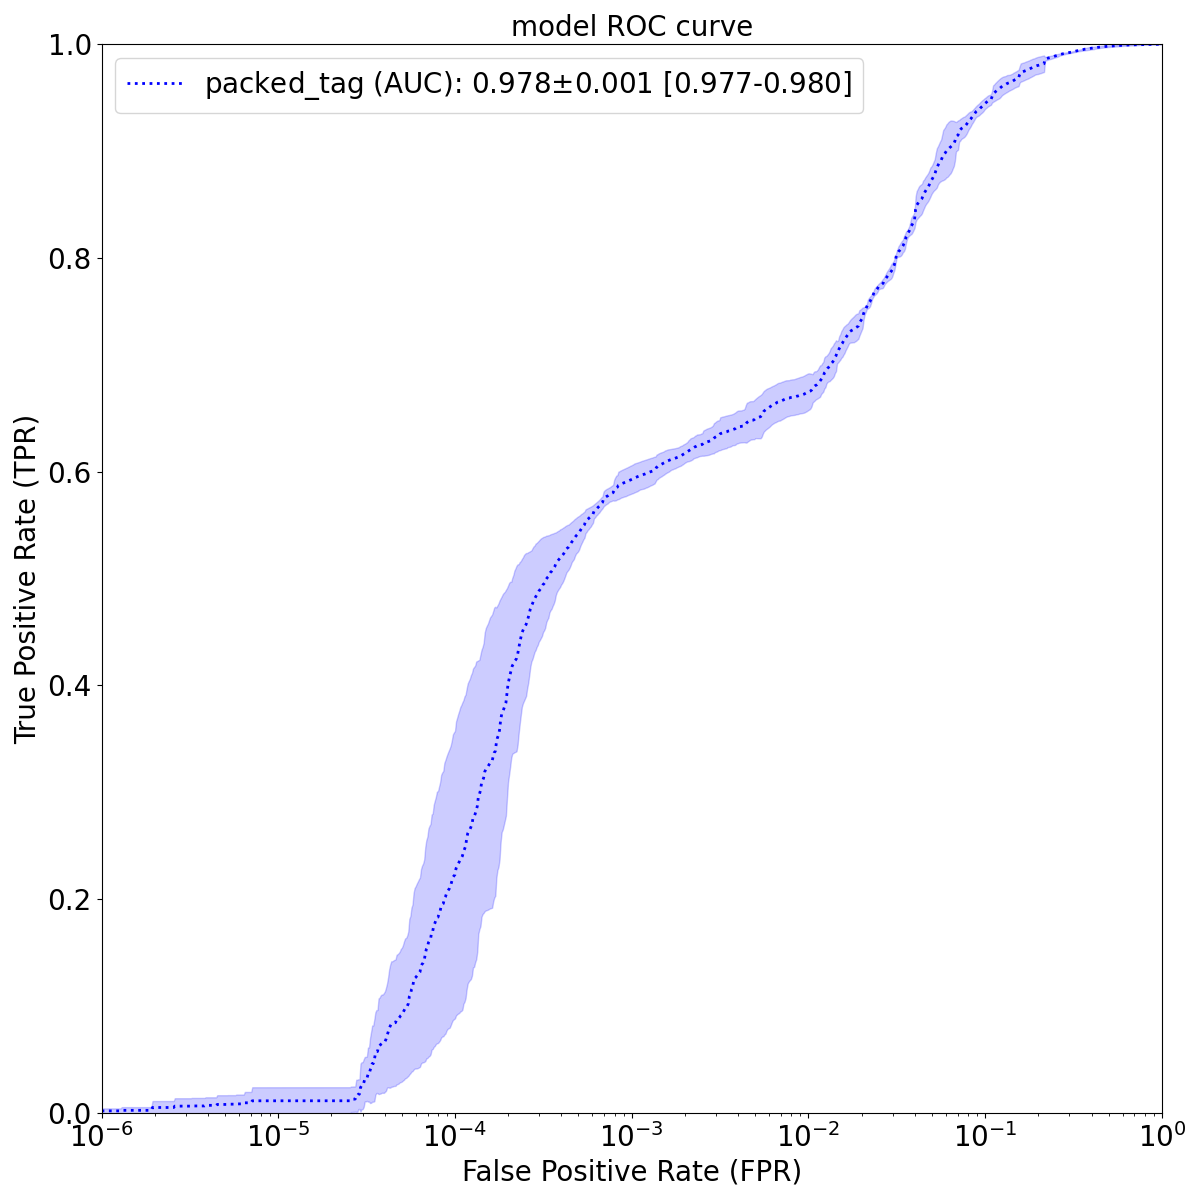
\includegraphics[width=0.6\textwidth]{./results/packed_tag_roc_aloha.png}
        \vspace*{-0.2cm}
        \caption{ROC curve and AUC statistics of \textBF{ALOHA} model for the \textbf{Packed Tag}. The line represents the \textit{mean} TPR at a given FPR, while the shaded region represents the \textit{standard deviation}. Statistics were computed over \textBF{3} training runs, each with random parameter initialization.}
        \label{fig:packedTagRocAloha}
    \end{figure}
}

\newcommand{\packedTagRocJointEmbedding}{
    \begin{figure}[H]
        \vspace*{-0.5cm}
        \centering
        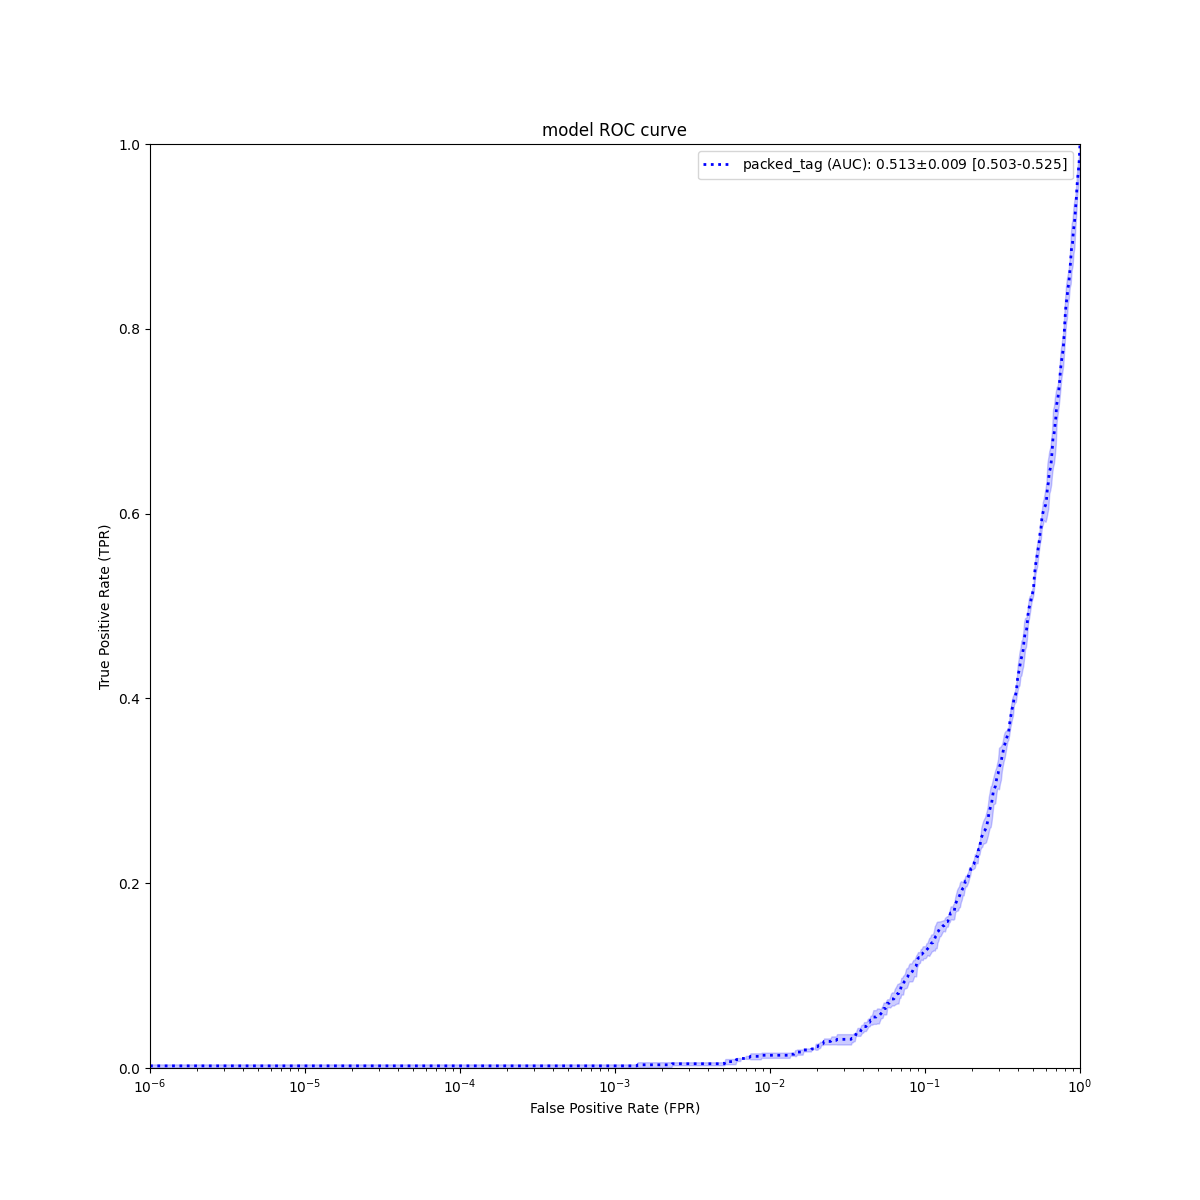
\includegraphics[width=0.6\textwidth]{./results/packed_tag_roc_jointEmbedding.png}
        \vspace*{-0.2cm}
        \caption{ROC curve and AUC statistics of \textBF{Joint Embedding} model for the \textbf{Packed Tag}. The line represents the \textit{mean} TPR at a given FPR, while the shaded region represents the \textit{standard deviation}. Statistics were computed over \textBF{3} training runs, each with random parameter initialization.}
        \label{fig:packedTagRocJointEmbedding}
    \end{figure}
}

\newcommand{\packedTagRocProposedMethod}{
    \begin{figure}[H]
        \vspace*{-0.5cm}
        \centering
        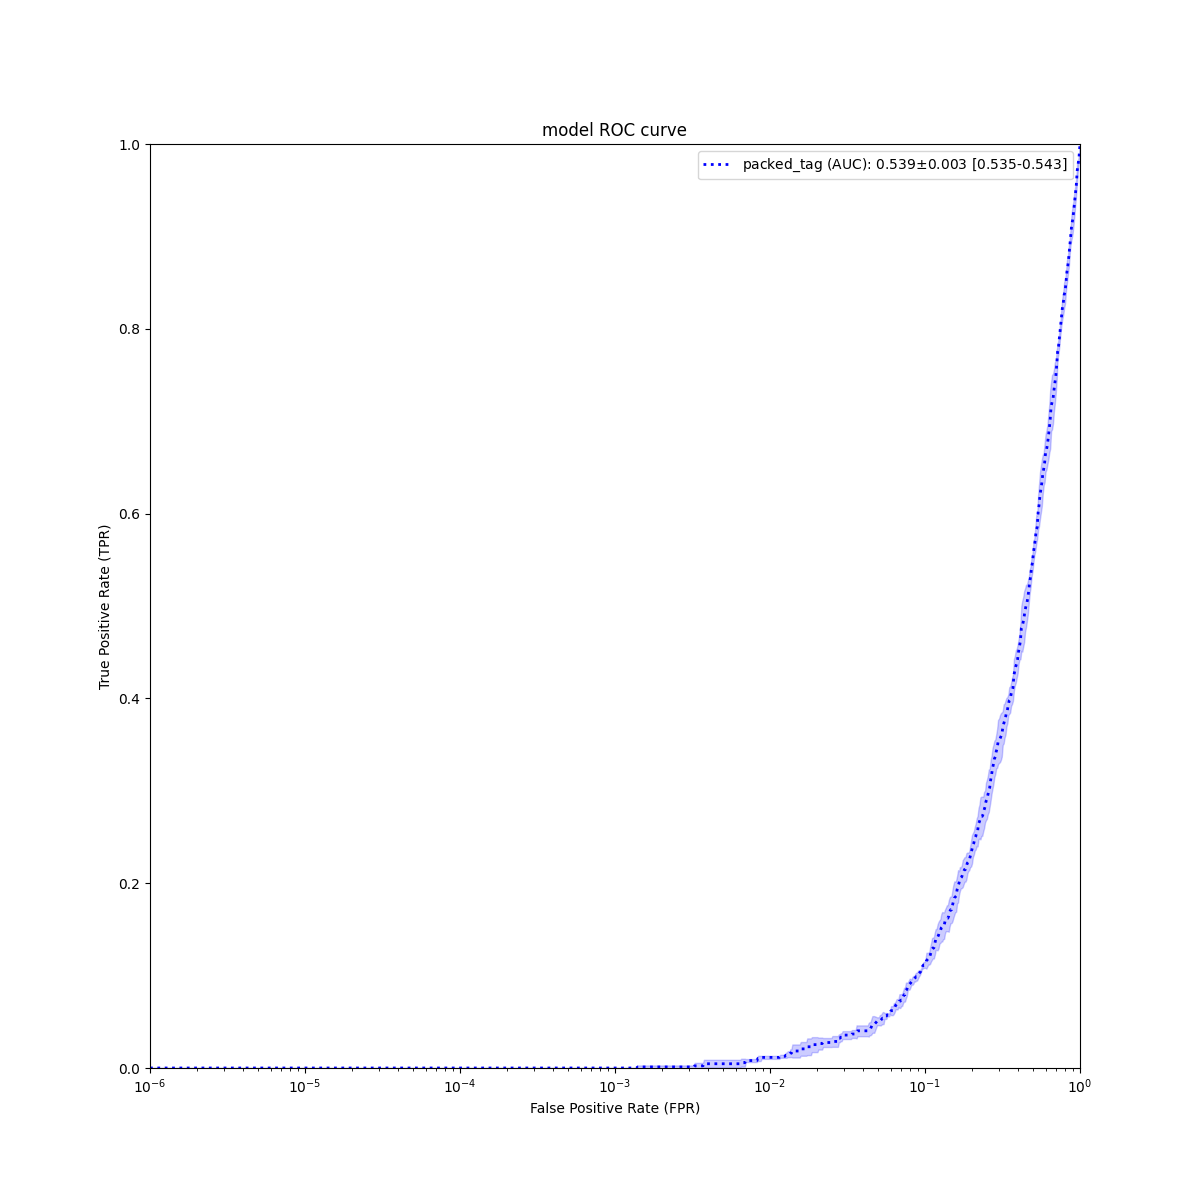
\includegraphics[width=0.6\textwidth]{./results/packed_tag_roc_proposedModel.png}
        \vspace*{-0.2cm}
        \caption{ROC curve and AUC statistics of \textBF{Proposed Model} for the \textbf{Packed Tag}. The line represents the \textit{mean} TPR at a given FPR, while the shaded region represents the \textit{standard deviation}. Statistics were computed over \textBF{3} training runs, each with random parameter initialization.}
        \label{fig:packedTagRocProposedModel}
    \end{figure}
}
